\documentclass[a4paper, 11pt]{article}

\setcounter{tocdepth}{3}
\setcounter{secnumdepth}{3}

\usepackage{comment} % enables the use of multi-line comments (\ifx \fi) 
\usepackage{lipsum} %This package just generates Lorem Ipsum filler text. 
\usepackage{fullpage} % changes the margin
\usepackage[utf8]{inputenc}
\usepackage{gensymb}
\usepackage{graphicx}
\usepackage{booktabs}% http://ctan.org/pkg/booktabs
\usepackage{makecell}
\usepackage{tabularx}
\usepackage[table]{xcolor}
\usepackage{array}
\usepackage{wrapfig}
\usepackage{subcaption}
\usepackage{csquotes}
\usepackage{lscape}
\usepackage{afterpage}
\usepackage{geometry}
\usepackage{listingsutf8}
\usepackage{chngcntr}
\usepackage{multicol}
\usepackage{xcolor}
\usepackage{pifont}
\usepackage{outlines}
\usepackage{booktabs}% http://ctan.org/pkg/booktabs



\counterwithin{figure}{section}

\AtBeginDocument{\counterwithin{lstlisting}{section}}

\geometry{a4paper, margin=1in}

\renewcommand{\figurename}{Abb.}
\renewcommand{\tablename}{Tabelle}
\renewcommand*{\thead}[1]{\bfseries #1}
\renewcommand{\contentsname}{Inhalt}
\renewcommand{\listfigurename}{Abbildungsverzeichnis}

\newcommand{\code}[1]{\texttt{#1}}
\newcommand \tabitem{\makebox[1em][r]{\textbullet~}}


\definecolor{lightgray}{rgb}{.9,.9,.9}
\definecolor{darkgray}{rgb}{.4,.4,.4}
\definecolor{purple}{rgb}{0.65, 0.12, 0.82}
\definecolor{darkgreen}{rgb}{0.05,0.56,0.06}


\lstset{frame=tlrb,
	language=Java,
	captionpos=b,
	aboveskip=3mm,
	belowskip=3mm,
	showstringspaces=false,
	columns=flexible,
	basicstyle={\small\ttfamily},
	numbers=left,
	numberstyle=\tiny\color{gray},
	keywordstyle=\color{blue},
	commentstyle=\color{violet},
	stringstyle=\color{darkgreen},
	breaklines=true,
	breakatwhitespace=true,
	tabsize=3,
	literate=%
	{Ö}{{\"O}}1
	{Ä}{{\"A}}1
	{Ü}{{\"U}}1
	{ß}{{\ss}}1
	{ü}{{\"u}}1
	{ä}{{\"a}}1
	{ö}{{\"o}}1
}


\begin{document}

\newgeometry{top=0in, bottom=0in}
\title{Zusammenfassung Sicheres Programmieren FS2019}
\author{Alex Neher}
\maketitle

\tableofcontents

\newpage
\graphicspath{{./Pictures/}}

\restoregeometry

\section{Requirements Engineering}

\begin{figure}[htb]
	\centering
	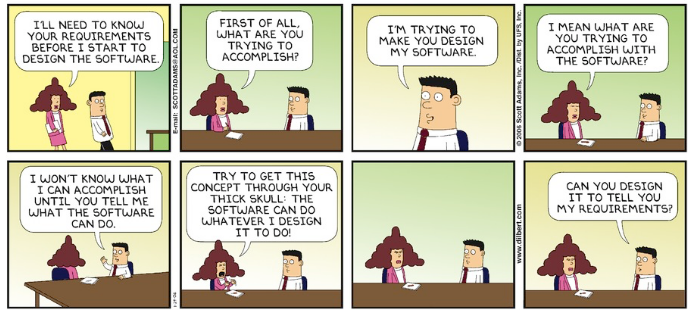
\includegraphics[keepaspectratio=true,height=15\baselineskip]{req_engineering.png}
	\caption{Requirements Engineering in der Praxis}
    \label{fig:req_eng}
\end{figure}

\begin{quote}
     \centering
     \blockquote{Requirements engineering refers to the process of formulating, documenting and maintaining software requirements and to the subfield of Software Engineering concerned with the process}
\end{quote}


Dieser Prozess des Requirements Engineerings wird meist von einem Business Analyst geleitet. Wieso nicht direkt vom Programmierer selbst? Das hat mehrere Gründe. 

\begin{wrapfigure}[15]{R}{0.5\textwidth}
    \centering
    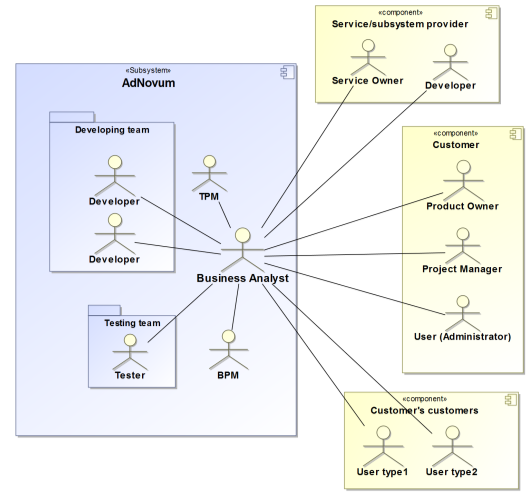
\includegraphics[keepaspectratio=true,height=15\baselineskip]{ba.png}
    \caption{Der Business Analyst ist die Ansprechsperson für alle Parteien}
    \label{fig:datawarehouse}
\end{wrapfigure}

\begin{outline}
    \1 Muss extensives Wissen über das Business-Feld der einzusetzenden Lösung haben
        \2 Regulationen und Richtlinien müssen eingehlaten werden
        \2 Muss Fragen von Devs über Funktionalitäten beantworten könne, auch wenn der verantwortliche Stakeholder evtl. nicht verfügbar ist
        \2 Stakeholder sehen evtl. nicht das 'Big Picture'
        \2 Somit kann der Analyst die Kontakperson sowohl für Devs wie auch für Business Stakeholder sein.
    \1 Ein Business Analyst kann einfacher klare Requirements und vollständige Spezifikationen entwickeln. Dies bringt einige Vorteile
        \2 Ermöglicht klare estimates
        \2 Ermöglicht bessere und exaktere Planung
        \2 Führt zu schnellerer Entwicklung/Durchführung des Projekts, da die Devs weniger Fragen haben
        \2 Führt zu höherer Endqualität
        \2 Führt zu weniger Change Requests während der Entwicklung
\end{outline}

\vspace{5px}

Ein Business Analyst hat sich eingehend mit dem Feld der Business Analyse auseinandergesetzt. Business Analyse ist das Feld, das sich damit beschäftigt, was Firmen überhaupt brauchen. Anschliessend entwickelt der Business Analyst Lösungen, die diese Bedürfnisse abdecken. Im Feld der Informatik ist diese Lösung meist eine Software, aber prinzipiell kann es auch z.B. eine Prozess- oder Organisationsänderung sein.

\vspace{10px}

Der Business Analyst ist während des gesamten Lifecycles eines Projekts daran beteiligt, nicht nur bis die Requirements stehen. 

\vspace{60px}

\begin{tabularx}{\textwidth}{|p{5cm}|X|}
	\hline 
    \thead{Projektphase} & \thead{Aufgaben} \\
    \hline
    Requirement Analyse & 
        \tabitem Stakeholder-Analyse \newline
        \tabitem Dokumenten-Analyse \newline
        \tabitem Erhebung der Anforderungen \newline
        \tabitem Workshops / Interviews mit Stakeholder \newline
        \tabitem Business- und User-Requirement Analyse \newline
        \tabitem Auflistung und Priorisierung der Use Cases 
        \\
    \hline
    Design & 
        \tabitem Detaillierte Spezifikationen von Business Prozessen, Aktoren, Use Cases und Interfaces \newline
        \tabitem GUI Design \newline
        \tabitem Review der Spezifikationen \newline
        \tabitem Abnahme der Spezifikationen
    \\
    \hline
    Implementation & 
        \tabitem Walkthrough der Spezifikationen mit TPL (??) und Devs \newline
        \tabitem Support der Devs \newline
        \tabitem Klärung von allfälligen neuen Punkten mit den Business Stakeholder \newline
        \tabitem Change Management
    \\
    \hline
    Testing & 
        \tabitem Test Support \newline
        \tabitem Klärung von allfälligen Defekten \newline
        \tabitem Klärung von allfälligen neuen Issues \newline
        \tabitem Change Management
    \\
    \hline
    Evolution & 
        \tabitem Analyse der Change Requests \newline
        \tabitem Kundensupport \newline
        \tabitem 'Aufräumen' der Dokumentation
    \\
    \hline
\end{tabularx}

\end{document}

